\section{Informal Discussion on Our Variable Decision Boundary}
\label{vdb}
In the introduction, we claim that in traditional supervised learning $\vtheta$ gives a fixed decision boundary, while our $\vtheta$ gives a variable decision boundary. Here we informally discuss this claim.

Denote the input space $\scrX$ and output space $\scrY$. 
A decision boundary is simply a mapping $f: \scrX \rightarrow \scrY$.
Let $\Theta$ be a model class e.g $\mathbb{R}^d$.
Now consider a family of parametrized functions $g_\vtheta: \scrX \rightarrow \scrY$, where $\vtheta\in \Theta$.
In the context of deep learning, $g$ is the neural network architecture and $\vtheta$ contains the parameters. 
We say that $f$ is a fixed decision boundary w.r.t. $g$ and $\Theta$
if there exists $\vtheta\in\Theta$ s.t. $f(x) = g_\vtheta(x)$ for every $x\in\scrX$,
and a variable decision boundary if for every $x\in\scrX$, there exists $\vtheta\in\Theta$ s.t. $f(x) = g_\vtheta(x)$.
Note how selection of $\vtheta$ can depend on $x$ for a variable decision boundary, and cannot for a fixed one. It is then trivial to verify that our claim is true under those definitions.

A critical reader might say that with an arbitrarily large model class, can't every decision boundary be fixed?
Yes, but this is not the end of the story.
Let $d = \dim(\scrX) \times \dim(\scrY)$, and consider the enormous model class $\Theta' = \R^d$ which is capable of representing all possible mappings between $\scrX$ and $\scrY$.
Let $g'_{\vtheta'}$ simply be the mapping represented by $\vtheta'\in\Theta'$.
A variable decision boundary w.r.t. $g$ and $\Theta$ then indeed must be a fixed decision boundary w.r.t. $g'$ and $\Theta'$, but we would like to note two things.
First, without any prior knowledge, generalization in $\Theta'$ is impossible with any finite amount of training data; 
reasoning about  $g'$ and $\Theta'$ is most likely not productive from an algorithmic point of view, and the concept of a variable decision boundary is to avoid such reasoning.
Second, selecting $\vtheta$ based on $x$ for a variable decision boundary can be thought of as ``training" on all points $x\in\R^d$; however, ``training" only happens when necessary, for the $x$ that it actually encounters. 

Altogether, the concept of a variable decision boundary is different from what can be described
by traditional learning theory. 
A formal discussion is beyond the scope of this paper and might be of interest to future work.

\section{Computational Aspects of Our Method}
\label{computational}
At test time, our method is $2~\times$
\texttt{batch\_size}
$\times$
\texttt{number\_of\_iterations} 
times slower than regular testing, 
which only performs a single forward pass for each sample. 
As the first work on Test-Time Training, this paper is not as concerned about computational efficiency as improving robustness, but here we provide two potential solutions that might be useful, but have not been thoroughly verified.
The first is to use the thresholding trick on $l_s$, introduced as a solution for the small batches problem in the method section. For the models considered in our experiments, roughly $80\%$ of the test instances fall below the threshold, so Test-Time Training can only be performed on the other $20\%$ without much effect on performance, because those $20\%$ contain most of the samples with wrong predictions.
The second is to reduce the \texttt{number\_of\_iterations} of test-time updates. For the online version, the \texttt{number\_of\_iterations} is already 1, so there is nothing to do. For the standard version, we have done some preliminary experiments setting \texttt{number\_of\_iterations} to 1 (instead of 10) and learning rate to 0.01 (instead of 0.001), and observing results almost as good as the standard hyper-parameter setting.
A more in depth discussion on efficiency is left for future works, which might, during training, explicitly make the model amenable to fast updates.

\section{Proofs}
Here we prove the theoretical results in the main paper.
\subsection{The Toy Problem}
The following setting applies to the two lemmas; this is simply the setting of our toy problem, reproduced here for ease of reference.

\pagebreak
Consider a two layer linear network parametrized by $\mA\in\R^{h\times d}$ (shared) and $\vv, \vw\in\R^h$ (fixed) for the two heads, respectively.
Denote $x\in\R^d$ the input and $y_1, y_2\in\R$ the labels for the two tasks, respectively.
For the main task loss
\begin{equation}
l_m(\mA; \vv) = \frac{1}{2}\left(y_1 - \vv^\top \mA x\right)^2,
\end{equation}
and the self-supervised task loss
\begin{equation}
l_s(\mA; \vw) = \frac{1}{2}\left(y_2 - \vw^\top \mA x\right)^2,
\end{equation}
Test-Time Training yields an updated matrix
\begin{equation}
\mA' \leftarrow \mA - \eta\left( y_2-\vw^\top \mA x \right) \left(-\vw x^\top \right),
\end{equation}
where $\eta$ is the learning rate.

{\lemma \label{lemma_lr}
Following the exposition of the main paper, let
\begin{equation}
\eta\opt  = \frac{(y_1 - v^\top A x)}{(y_2 - w^\top A x) v^\top w x^\top x}.
\end{equation}
Assume $\eta\opt \in [\epsilon, \infty)$ for some $\epsilon > 0$.
Then for any $\eta \in (0, \epsilon]$,
we are guaranteed an improvement on the main loss i.e. $l_m(\mA') < l_m(\mA)$.
}
{\proof
From the exposition of the main paper, we know that
$$l_m(\mA - \eta\opt \grad l_s\mA)) = 0,$$
which can also be derived from simple algebra.
Then by convexity, we have
\begin{align}
l_m&\paren{\mA - \eta \grad l_s(\mA)}\\
&= l_m\paren{\paren{1 - \frac{\eta}{\eta\opt}} \mA 
	+ \frac{\eta}{\eta\opt}(\mA - \eta\opt \grad l_s(\mA))}  \\
&\leq \paren{1 - \frac{\eta}{\eta\opt}} l_m(\mA) + 0 \\
&\leq \paren{1 - \frac{\eta}{\epsilon}} l_m(\mA)\\
&< l_m(\mA),
\end{align}
where the last inequality uses the assumption that $l_m(\mA)>0$, which holds
because $\eta\opt > 0$.}
{\lemma \label{lemma_sign}
Define
$\langle \mU, \mV \rangle
= \text{vec} \left(\mU\right)^\top \text{vec} \left(\mV \right)$ 
i.e. the Frobenious inner product, then
\begin{equation}
\sign \left(\eta\opt\right) = \sign \left(\langle \grad l_m(\mA), \grad l_s(\mA)\rangle\right).
\end{equation}
}
{\proof By simple algebra,
\begin{align*}
&\langle\grad  l_m(\mA), \grad l_s(\mA)\rangle \\
&= 
    \langle\left( y_1-\vv^\top \mA x \right)\left(-\vv x^\top \right),
    \left( y_2-\vw^\top \mA x \right)\left(-\vw x^\top \right)\rangle\\
&= \left( y_1-\vv^\top \mA x \right)\left( y_2-\vw^\top \mA x \right)
\Tr \left( x \vv^\top \vw x^\top \right)\\
&= \left( y_1-\vv^\top\mA x \right)\left( y_2-\vw^\top\mA x \right) 
\vv^\top \vw x^\top x,
\end{align*}
}
which has the same sign as $\eta\opt$.

\subsection{Proof of Theorem 1}
\label{main_theorem_proof}
For any $\eta$, by smoothness and convexity,
\begin{align*}
\label{proof_first_eq}
&l_m(x,y; \vtheta(x))
= l_m(x,y; \vtheta - \eta \grad l_s(x; \vtheta))\\
&\leq l_m(x,y; \vtheta) 
+ \eta \langle \grad l_m(x, y; \vtheta), \grad l_s(x, \vtheta) \rangle \\
&\qquad+ \frac{\eta^2\beta}{2} \norm{\grad l_s(x; \vtheta)}^2.
\end{align*}
Denote
$$\eta\opt = \frac{\langle \grad l_m(x, y; \vtheta), \grad l_s(x, \vtheta) \rangle}
{\beta \norm{\grad l_s(x; \vtheta)}^2}.$$ 
Then \autoref{proof_first_eq} becomes
\begin{align}
&l_m(x,y; \vtheta - \eta\opt \grad l_s(x; \vtheta))\\
&\leq l_m(x,y; \vtheta) 
- \frac{\langle \grad l_m(x, y; \vtheta), \grad l_s(x, \vtheta) \rangle^2}
{2\beta \norm{\grad l_s(x; \vtheta)}^2}.
\end{align}
And by our assumptions on the gradient norm 
and gradient inner product,
\begin{align}
\label{proof_second_eq}
l_m(x,y; \vtheta)  - l_m(x,y; \vtheta - \eta\opt \grad l_s(x; \vtheta)) \geq\frac{\eps^2}{2\beta G^2}.
\end{align}
Because we cannot observe $\eta\opt$ in practice, we instead use a fixed learning rate $\eta = \frac{\eps}{\beta G^2}$, as stated in Theorem 1.
Now we argue that this fixed learning rate still improves performance on the main task.

By our assumptions, $\eta\opt \geq \frac{\eps}{\beta G^2}$, 
so $\eta \in (0, \eta\opt]$.
Denote $\vg = \grad l_s(x; \vtheta)$, then by convexity of $l_m$,
\begin{align}
&l_m(x,y; \vtheta(x))
= l_m(x,y; \vtheta - \eta \vg)\\
&= l_m\paren{x,y; 
	\paren{1 - \frac{\eta}{\eta\opt}} \vtheta +
	\frac{\eta}{\eta\opt} \paren{\vtheta - \eta\opt \vg}} \\
&\leq \paren{1 - \frac{\eta}{\eta\opt}} l_m(x,y; \vtheta) 
+ \frac{\eta}{\eta\opt} l_m(x,y; \vtheta - \eta\opt g)
\end{align}
Combining with \autoref{proof_second_eq}, we have
\begin{align*}
l_m(x,y; \vtheta(x))
&\leq \paren{1 - \frac{\eta}{\eta\opt}} l_m(x,y; \vtheta) \\
&\qquad
+ \frac{\eta}{\eta\opt} \paren{l_m(x,y; \vtheta) - \frac{\eps^2}{2\beta G^2}} \\
&= l_m(x,y; \vtheta) - \frac{\eta}{\eta\opt}\frac{\eps^2}{2\beta G^2}
\end{align*}
Since $\eta / \eta\opt > 0$, we have shown that
\begin{align}
l_m(x,y; \vtheta)  - l_m(x,y; \vtheta(x)) > 0.
\end{align}


\pagebreak

\section{Additional Results on the Common Corruptions Dataset}
\label{results_additional}
For table aethetics, we use the following abbreviations:
B for baseline, JT for joint training, TTT for Test-Time Training standard version, and TTT-Online for online Test-Time Training i.e. the online version.

We have abbreviated the names of the corruptions, in order: original test set, Gaussian noise, shot noise, impulse noise, defocus blur, glass blue, motion blur, zoom blur, snow, frost, fog, brightness, contrast, elastic transformation, pixelation, and JPEG compression. 

\subsection{Results Using Batch Normalization}
As discussed in the results section, Batch Normalization (BN) is ineffective for small batches, which are the inputs for Test-Time Training (both standard and online version) since there is only one sample available when forming each batch; therefore, our main results are based on a ResNet using Group Normalization (GN). 
\autoref{figure:bn} and \autoref{table:bn} show results of our method on CIFAR-10-C level 5, with a ResNet using Batch Normalization (BN). These results are only meant to be a point of reference for the curious readers.

In the early stage of this project, we have experimented with two potential solutions to the small batches problem with BN.  The naive solution is to fix the BN layers during Test-Time Training. but this diminishes the performance gains since there are fewer shared parameters. 
The better solution, adopted for the results below, is hard example mining: instead of updating on all inputs, we only update on inputs that incur large self-supervised task loss $l_s$,
where the large improvements might counter the negative effects of inaccurate statistics.

Test-Time Training (standard version) is still very effective with BN. 
In fact, some of the improvements are quite dramatic, such as on contrast (34\%), defocus blue (18\%) and Gaussian noise (22\% comparing to joint-training, and 16\% comparing to the baseline). Performance on the original distribution is still almost the same, and the original error with BN is in fact slightly lower than with GN, and takes half as many epochs to converge.

We did not further experiment with BN because of two reasons:
1) The online version does not work with BN, because the problem with inaccurate batch statistics is exacerbated when training online for many (e.g. 10000) steps. 2) The baseline error for almost every corruption type is significantly higher with BN than with GN. Although unrelated to the main idea of our paper, we make the interesting note that \emph{GN significantly improves model robustness}.

\subsection{Additional Baseline: Adversarial Logit Pairing}
As discussed in the results section, \citet{hendrycks2019benchmarking} point to Adversarial Logit Pairing (ALP) \citep{kannan2018adversarial} as an effective method for improving model robustness to corruptions and perturbations, even though it was designed to defend against adversarial attacks. 
We take ALP as an additional baseline on all benchmarks based on CIFAR-10 (using GN), following the training procedure in \citet{kannan2018adversarial} and their recommended hyper-parameters.
The implementation of the adversarial attack comes from the codebase of \citet{ding2019advertorch}. 
We did not run ALP on ImageNet because the two papers we reference for this method, \citet{kannan2018adversarial} and \citet{hendrycks2019benchmarking}, did not run on ImageNet or make any claim or recommendation.

\subsection{Results on CIFAR-10-C and ImageNet-C, Level 5}
\autoref{table:full_c10c} and \autoref{table:imgnet} correspond to the bar plots in the results section. Two rows of \autoref{table:full_c10c} have been presented as \autoref{table:uda} in the main text.

\begin{figure*}
	\centering
	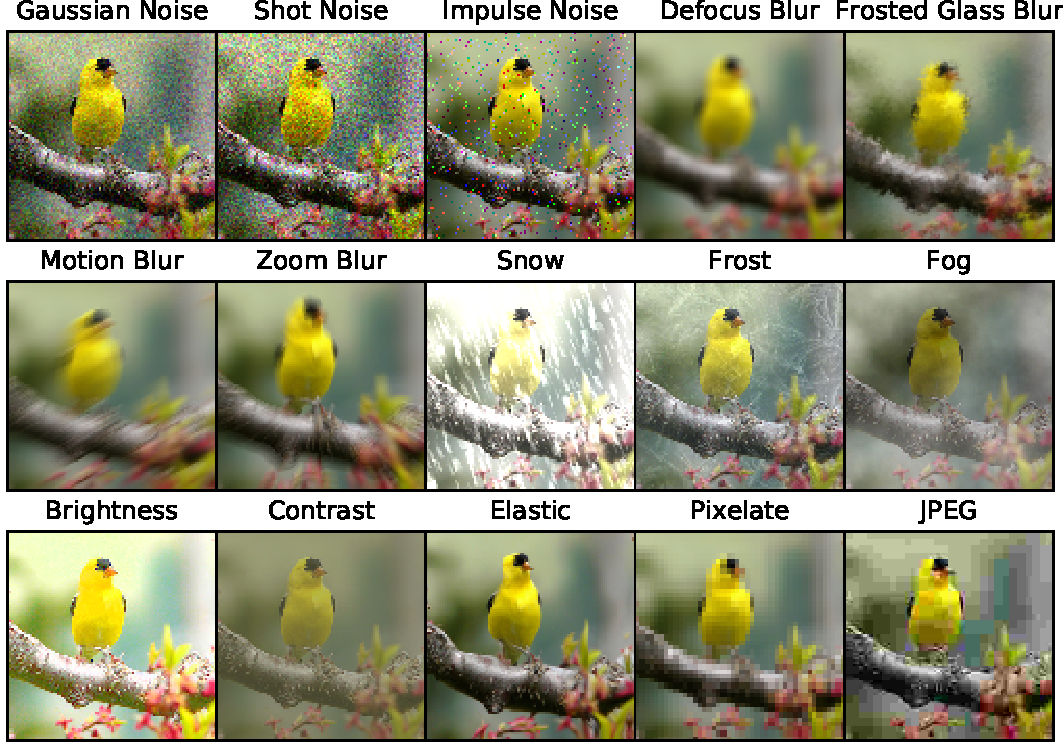
\includegraphics[width=0.6\textwidth]{plots/distorted}
	\caption{
		Sample images from the Common Corruptions Benchmark, taken from the original paper by \citet{hendrycks2019benchmarking}.
	}
\end{figure*}

\begin{figure*}[ht]
	\centering
	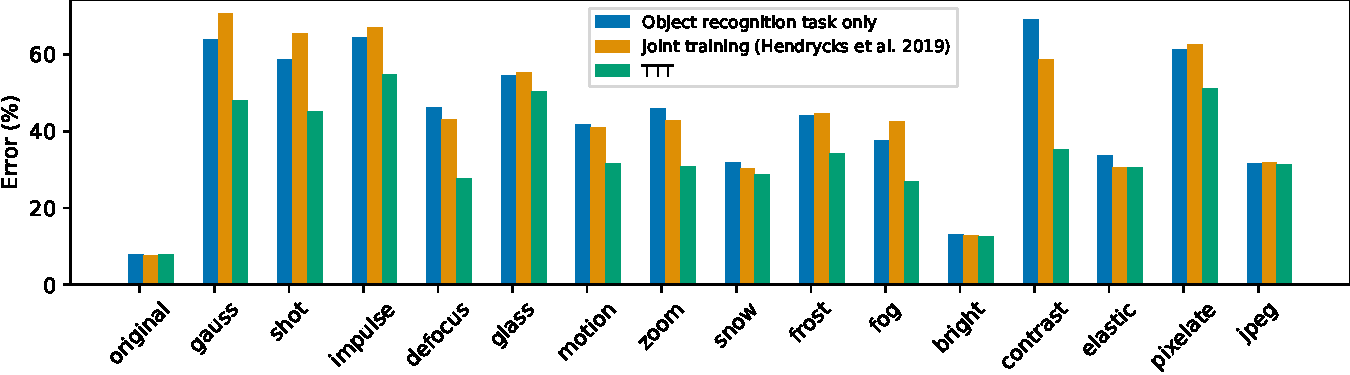
\includegraphics[width=1.0\textwidth]{plots/C10C_layer2_5_bn_expand_final}
	\caption{
		Test error (\%) on CIFAR-10-C, level 5, ResNet-26 with Batch Normalization.
	\label{figure:bn}
	}
\end{figure*}

\begin{table*}[ht]
	\footnotesize
	\begin{center}
		{
			\setlength\tabcolsep{3.5pt}
			\begin{tabular}{c|c|c|c|c|c|c|c|c|c|c|c|c|c|c|c|c}
				\hline
				& orig& gauss& shot& impul& defoc& glass& motn& zoom& snow& frost& fog& brit& contr& elast& pixel& jpeg\\
				\hline
				B & 7.9& 63.9& 58.8& 64.3& 46.3& 54.6& 41.6& 45.9& 31.9& 44.0& 37.5& 13.0& 69.2& 33.8& 61.4& 31.7\\
				\hline
				JT & 7.5& 70.7& 65.6& 67.2& 43.1& 55.4& 40.9& 42.7& 30.3& 44.5& 42.5& 12.7& 58.6& 30.7& 62.6& 31.9\\
				\hline
				TTT & 7.9& 47.9& 45.2& 54.8& 27.6& 50.4& 31.5& 30.9& 28.7& 34.3& 26.9& 12.6& 35.2& 30.6& 51.2& 31.3\\
				\hline
			\end{tabular}
		}
	\end{center}
	\vspace{-2ex}
	\caption{
		Test error (\%) on CIFAR-10-C, level 5, ResNet-26 with Batch Normalization.
	}
	\label{table:bn}
\end{table*} 

\subsection{Results on CIFAR-10-C, Levels 1-4}
The following bar plots and tables are on levels 1-4 of CIFAR-10-C.
The original distribution is the same for all levels, so are our results on the original distribution.

\subsection{Direct Comparison with \citet{hendrycks2019using}}
\label{reviewer_stuff}
The following comparison has been requested by an anonymous reviewer for our final version.
Our joint training baseline is based on \citet{hendrycks2019using}, but also incorporates some architectural changes (see below). We found these changes improved the robustness of our method, and felt that it was important to give the baseline the same benefit. Note that our joint training baseline overall performs better than Hendrycks: Compare Table S2 to Figure 3 of \citet{hendrycks2019using} (provided by the authors), our baseline has average error of 22.8\% across all corruptions and levels, while their average error is 28.6\%. 

Summary of architectural changes: 1) Group Normalization (GN) instead of Batch Normalization (BN). For completeness, the results with BN are provided in Table S1; c.f. GN results in Table S2 which significantly improves robustness, with or without self-supervision. 2) We split after the second residual group, while they split after the third residual group right before the linear layer. This consistently gives about 0.5\% - 1\% improvement. 3) We use a ResNet-26, while they use a 40-2 Wide ResNet. But our baseline still performs better than their method even though our network is 4x smaller, due to the two tricks above.

\newpage
\begin{table*}[ht]
	\footnotesize
	\begin{center}
		{
			\setlength\tabcolsep{3.5pt}
			\begin{tabular}{c|c|c|c|c|c|c|c|c|c|c|c|c|c|c|c|c}
				\hline
				& orig& gauss& shot& impul& defoc& glass& motn& zoom& snow& frost& fog& brit& contr& elast& pixel& jpeg\\
				\hline
				B & 8.9& 50.5& 47.2& 56.1& 23.7& 51.7& 24.3& 26.3& 25.6& 34.4& 28.1& 13.5& 25.0& 27.4& 55.8& 29.8\\
				\hline
				JT & 8.1& 49.4& 45.3& 53.4& 24.2& 48.5& 24.8& 26.4& 25.0& 32.5& 27.5& 12.6& 25.3& 24.0& 51.6& 28.7\\
				\hline
				TTT & 7.9& 45.6& 41.8& 50.0& 21.8& 46.1& 23.0& 23.9& 23.9& 30.0& 25.1& 12.2& 23.9& 22.6& 47.2& 27.2\\
				\hline
				TTT-Online & 8.2& 25.8& 22.6& 30.6& 14.6& 34.4& 18.3& 17.1& 20.0& 18.0& 16.9& 11.2& 15.6& 21.6& 18.1& 21.2\\
				\hline
				UDA-SS & 9.0& 28.2& 26.5& 20.8& 15.6& 43.7& 24.5& 23.8& 25.0& 24.9& 17.2& 12.7& 11.6& 22.1& 20.3& 22.6\\
				\hline
				ALP & 16.5& 22.7& 22.9& 28.3& 25.0& 25.6& 27.4& 23.1& 25.2& 27.2& 64.8& 21.7& 73.6& 23.0& 20.2& 18.9\\
				\hline
			\end{tabular}
		}
	\end{center}
	\vspace{-2ex}
	\caption{
		Test error (\%) on CIFAR-10-C, level 5, ResNet-26.
	}
\label{table:full_c10c}
\end{table*} 

\begin{table*}[ht]
	\footnotesize
	\begin{center}
		{
			\setlength\tabcolsep{3.5pt}
			\begin{tabular}{c|c|c|c|c|c|c|c|c|c|c|c|c|c|c|c|c}
				\hline
				& orig& gauss& shot& impul& defoc& glass& motn& zoom& snow& frost& fog& brit& contr& elast& pixel& jpeg\\
				\hline
				B & 68.9& 1.3& 2.0& 1.3& 7.5& 6.6& 11.8& 16.2& 15.7& 14.9& 15.3& 43.9& 9.7& 16.5& 15.3& 23.4\\
				\hline
				JT & 69.1& 2.1& 3.1& 2.1& 8.7& 6.7& 12.3& 16.0& 15.3& 15.8& 17.0& 45.3& 11.0& 18.4& 19.7& 22.9\\
				\hline
				TTT & 69.0& 3.1& 4.5& 3.5& 10.1& 6.8& 13.5& 18.5& 17.1& 17.9& 20.0& 47.0& 14.4& 20.9& 22.8& 25.3\\
				\hline
				TTT-Online & 68.8& 26.3& 28.6& 26.9& 23.7& 6.6& 28.7& 33.4& 35.6& 18.7& 47.6& 58.3& 35.3& 44.3& 47.8& 44.3\\
				\hline
			\end{tabular}
		}
	\end{center}
	\vspace{-2ex}
	\caption{
		Test accuracy (\%) on ImageNet-C, level 5, ResNet-18.
	}
	\label{table:imgnet}
\end{table*} 

\newpage
\begin{figure*}[ht]
	\centering
	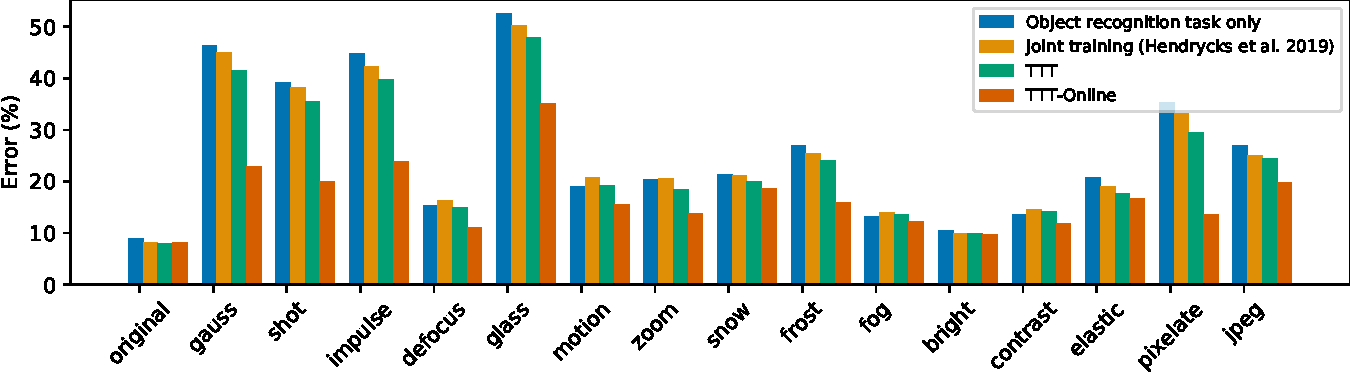
\includegraphics[width=1.0\textwidth]{plots/C10C_layer2_4_gn_expand_final}
	\vspace{-4ex}
	\caption{
		Test error (\%) on CIFAR-10-C, level 4.
		See the results section for details.
	}
	\vspace{4ex}
\end{figure*}

\begin{table*}[ht]
	\footnotesize
	\begin{center}
		{
			\setlength\tabcolsep{3.5pt}
			\begin{tabular}{c|c|c|c|c|c|c|c|c|c|c|c|c|c|c|c|c}
				\hline
				& orig& gauss& shot& impul& defoc& glass& motn& zoom& snow& frost& fog& brit& contr& elast& pixel& jpeg\\
				\hline
				B & 8.9& 46.4& 39.2& 44.8& 15.3& 52.5& 19.1& 20.5& 21.3& 26.9& 13.3& 10.5& 13.7& 20.8& 35.3& 26.9\\
				\hline
				JT & 8.1& 45.0& 38.3& 42.2& 16.4& 50.2& 20.7& 20.5& 21.1& 25.4& 14.1& 10.0& 14.7& 19.0& 33.2& 25.1\\
				\hline
				TTT & 7.9& 41.5& 35.4& 39.8& 15.0& 47.8& 19.1& 18.4& 20.1& 24.0& 13.5& 10.0& 14.1& 17.7& 29.4& 24.5\\
				\hline
				TTT-Online & 8.2& 22.9& 20.0& 23.9& 11.2& 35.1& 15.6& 13.8& 18.6& 15.9& 12.3& 9.7& 11.9& 16.7& 13.6& 19.8\\
				\hline
				ALP & 16.5& 21.3& 20.5& 24.5& 20.7& 25.9& 23.7& 21.4& 24.2& 23.9& 42.2& 17.5& 53.7& 22.1& 19.1& 18.5\\
				\hline
			\end{tabular}
		}
	\end{center}
	\vspace{-2ex}
	\caption{
		Test error (\%) on CIFAR-10-C, level 4, ResNet-26.
	} 
\end{table*} 

\begin{figure*}[ht]
	\vspace{8ex}
	\centering
	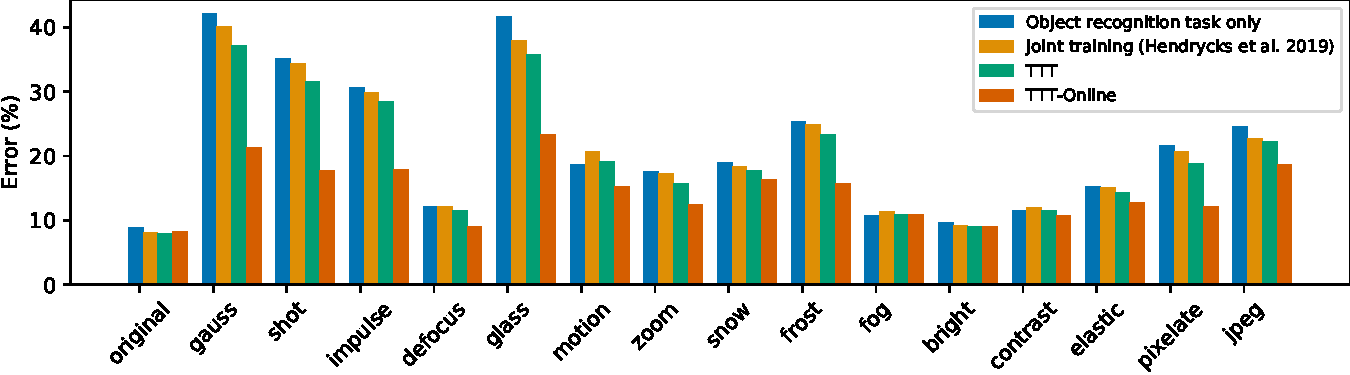
\includegraphics[width=1.0\textwidth]{plots/C10C_layer2_3_gn_expand_final}
	\vspace{-4ex}
	\caption{
		Test error (\%) on CIFAR-10-C, level 3.
		See the results section for details.
	}
\end{figure*}

\begin{table*}[ht]
	\vspace{4ex}
	\footnotesize
	\begin{center}
		{
			\setlength\tabcolsep{3.5pt}
			\begin{tabular}{c|c|c|c|c|c|c|c|c|c|c|c|c|c|c|c|c}
				\hline
				& orig& gauss& shot& impul& defoc& glass& motn& zoom& snow& frost& fog& brit& contr& elast& pixel& jpeg\\
				\hline
				B & 8.9& 42.2& 35.1& 30.7& 12.2& 41.7& 18.6& 17.5& 19.0& 25.3& 10.8& 9.7& 11.6& 15.3& 21.7& 24.6\\
				\hline
				JT & 8.1& 40.2& 34.4& 29.9& 12.2& 37.9& 20.8& 17.3& 18.4& 25.0& 11.4& 9.2& 12.0& 15.2& 20.8& 22.8\\
				\hline
				TTT & 7.9& 37.2& 31.6& 28.6& 11.5& 35.8& 19.1& 15.8& 17.8& 23.3& 11.0& 9.1& 11.6& 14.3& 18.9& 22.3\\
				\hline
				TTT-Online & 8.2& 21.3& 17.7& 17.9& 9.0& 23.4& 15.3& 12.5& 16.4& 15.8& 10.9& 9.0& 10.7& 12.8& 12.2& 18.7\\
				\hline
				ALP & 16.5& 20.0& 19.3& 20.5& 19.2& 21.2& 24.0& 20.5& 20.9& 24.2& 30.1& 16.6& 39.6& 20.9& 17.8& 18.0\\
				\hline
			\end{tabular}
		}
	\end{center}
	\caption{
		Test error (\%) on CIFAR-10-C, level 3, ResNet-26.
	} 
\end{table*}
 
\begin{figure*}[ht]
	\vspace{-1ex}
	\centering
	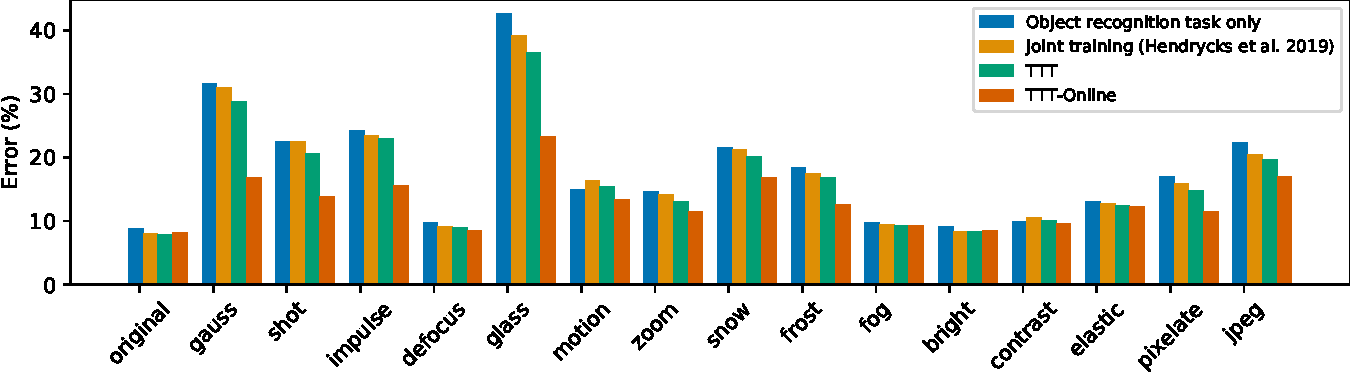
\includegraphics[width=1.0\textwidth]{plots/C10C_layer2_2_gn_expand_final}
	\vspace{-4ex}
	\caption{
		Test error (\%) on CIFAR-10-C, level 2.
		See the results section for details.
	}
	\vspace{-1ex}
\end{figure*}

\begin{table*}[ht]
	\footnotesize
	\begin{center}
		{
			\setlength\tabcolsep{3.5pt}
			\begin{tabular}{c|c|c|c|c|c|c|c|c|c|c|c|c|c|c|c|c}
				\hline
				& orig& gauss& shot& impul& defoc& glass& motn& zoom& snow& frost& fog& brit& contr& elast& pixel& jpeg\\
				\hline
				B & 8.9& 31.7& 22.6& 24.3& 9.9& 42.6& 14.9& 14.7& 21.7& 18.4& 9.8& 9.1& 10.0& 13.1& 17.1& 22.4\\
				\hline
				JT & 8.1& 31.0& 22.6& 23.4& 9.1& 39.2& 16.4& 14.2& 21.2& 17.5& 9.4& 8.3& 10.6& 12.8& 15.9& 20.5\\
				\hline
				TTT & 7.9& 28.8& 20.7& 23.0& 9.0& 36.6& 15.4& 13.1& 20.2& 16.9& 9.2& 8.3& 10.2& 12.5& 14.8& 19.7\\
				\hline
				TTT-Online & 8.2& 16.8& 13.8& 15.5& 8.5& 23.4& 13.3& 11.5& 16.8& 12.7& 9.4& 8.4& 9.7& 12.4& 11.5& 17.0\\
				\hline
				ALP & 16.5& 18.0& 17.2& 19.0& 17.8& 20.7& 21.2& 19.3& 19.0& 20.1& 22.4& 16.3& 29.2& 20.3& 17.4& 17.8\\
				\hline
			\end{tabular}
		}
	\end{center}
	\vspace{-2ex}
	\caption{
		Test error (\%) on CIFAR-10-C, level 2, ResNet-26.
	} 
\end{table*} 

\begin{figure*}[ht]
	\vspace{-1ex}
	\centering
	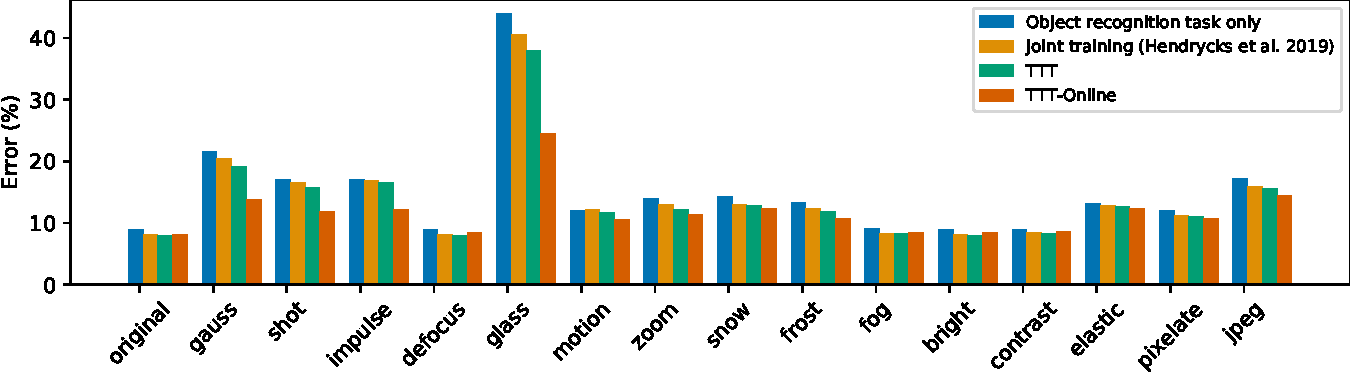
\includegraphics[width=1.0\textwidth]{plots/C10C_layer2_1_gn_expand_final}
	\vspace{-4ex}
	\caption{
		Test error (\%) on CIFAR-10-C, level 1.
		See the results section for details.
	}
	\vspace{-1ex}
\end{figure*}

\begin{table*}[ht]
	\footnotesize
	\begin{center}
		{
			\setlength\tabcolsep{3.5pt}
			\begin{tabular}{c|c|c|c|c|c|c|c|c|c|c|c|c|c|c|c|c}
				\hline
				& orig& gauss& shot& impul& defoc& glass& motn& zoom& snow& frost& fog& brit& contr& elast& pixel& jpeg\\
				\hline
				B & 8.9& 21.7& 17.1& 17.0& 9.0& 44.0& 12.1& 13.9& 14.3& 13.4& 9.2& 8.9& 9.0& 13.2& 12.0& 17.3\\
				\hline
				JT & 8.1& 20.4& 16.6& 16.9& 8.2& 40.5& 12.2& 13.0& 13.1& 12.3& 8.4& 8.1& 8.5& 12.9& 11.3& 15.9\\
				\hline
				TTT & 7.9& 19.1& 15.8& 16.5& 8.0& 37.9& 11.7& 12.2& 12.8& 11.9& 8.2& 8.0& 8.3& 12.6& 11.1& 15.5\\
				\hline
				TTT-Online & 8.2& 13.8& 11.9& 12.2& 8.5& 24.4& 10.5& 11.5& 12.4& 10.7& 8.5& 8.3& 8.6& 12.4& 10.7& 14.4\\
				\hline
				ALP & 17.0& 16.8& 17.6& 16.8& 20.9& 18.7& 19.0& 17.3& 17.5& 17.4& 16.1& 18.4& 20.4& 17.0& 17.2 & 17.5\\
				\hline
			\end{tabular}
		}
	\end{center}
	\vspace{-2ex}
	\caption{
		Test error (\%) on CIFAR-10-C, level 1, ResNet-26.
	} 
\end{table*} 